\chapter{Data}

\textit{
``Malone: Me father died of starvation in Ireland in the Black 47. Maybe you've heard of it.\\
Violet: The Famine?\\
Malone: No, the starvation. When a country is full of food, and exporting it, there can be no famine. Me father was starved dead; and I was starved out to America in me mother's arms''.\\
\textemdash\ ``Man and Superman'' by George Bernard Shaw
}

\section{Data Sources}
\vspace{0pt}
The data come from several primary sources, including (1) census data, (2) economic history research papers, and (3) original archival material from the National Library Ireland. Many materials only covered a few years, so this paper filled in the data by combining various materials. For example, regarding the price of oats, the data from 1821 to 1828 were obtained from Daniel's 2021 research, the data from 1829 to 1859 were obtained from Vamplew's 1980 research, and the data from 1850 to 1900 were obtained from Tuner's 1987 research. Below are all the variables and their sources.

\vspace{7pt}

\begin{spacing}{1}
\begin{ThreePartTable}
    \begin{TableNotes}
        \begin{spacing}{1}
        \vspace{7pt}
        \item[a] \textit{Irish census through history can be found in \href{https://www.cso.ie/en/statistics/historicalreports/}{CSO}. In 1851 census, there is a chapter discussing the differences between 1841 and 1851 to show the influence of famine.}
        \vspace{7pt}
        \item[b] \textit{Base on Documenting Ireland: Parliament, People and Migration. This article estimates the population in non-census years based on Irish immigration, mortality, and mid-year population data.}
        \vspace{7pt}
        \item[c] \textit{O = Oat, P = Potato, W = Wheat, B = Barley, the following abbreviations are the same}
        \vspace{7pt}
        \item[d] \textit{The potato data in this section are estimated from the agricultural stock situation during this period. Unfortunately, due to the lack of specific yields and the fact that grain yields per hectare are changing, for example, in 1837, the barley yield could reach 24.9 cwt, but the yield from 1847 to 1851 was only 18cwt.}
        \end{spacing}
    \end{TableNotes}
\begin{longtable}{cccc}
    \caption{Data and Sources} \\
    \toprule % 表格顶部线
    \textbf{Data} & \textbf{Details} & \textbf{Time} & \textbf{Sources} \\
    \midrule % 表格标题下方线
    \endfirsthead

    \caption[]{(Continued)} \\
    \toprule
    \textbf{Data} & \textbf{Details} & \textbf{Time} & \textbf{Sources} \\
    \midrule
    \endhead

    \midrule
    \multicolumn{4}{r}{\textit{Continued on next page}} \\
    \midrule
    \endfoot

    \bottomrule % 表格底部线
    \insertTableNotes
    \endlastfoot

    Population & Population & 1821, 1831, \ldots & Irish Census \tnote{a}\\
     & & Remain years & Estimated population \tnote{b}\\
    & & \\
    Wage & Craft man wage & 1821 \textendash\ 1900 & \citep{kennedy1997prices}\\
     & General wage & 1821 \textendash\ 1900 & \citep{d1989wages} \& \citep{bishop1915history}\\
    & & \\
    Ground Rent & Ground Rent & 1821 \textendash\ 1829 & \citep{m2013land} \\
     & & 1830 \textendash\ 1849 & \citep{geary2004trends} \\
     & & 1850 \textendash\ 1885 & \citep{guinnane1996bonds} \\
     & & 1886 \textendash\ 1900 & NA \\
    & & \\
    Tax & Tithe & 1821 \textendash\ 1900 & \citep{brynn1970irish} \& \citep{shaw2015economic} \\
    & & \\
    Grain Price & Oat & 1821 \textendash\ 1828 & \citep{daniel2021irish} \\
     & & 1829 \textendash\ 1859 & \citep{vamplew1980grain}\\ 
     & Potato & 1821 \textendash\ 1845 & \citep{kennedy1997prices} \\
     & Wheat & 1824 \textendash\ 1837 & Southampton library\\
     & Barley & 1821 \textendash\ 1828 & \citep{clark2004price} \\
     & O. P. W. B. \tnote{c} & 1840 \textendash\ 1900 & \citep{barrington1926review} \\
     & O. P. & 1821 \textendash\ 1850 & \citep{kennedy1997prices} \\
     & Agriculture index & 1850 \textendash\ 1900 & \citep{turner1987towards}\\
    & & \\

    Plant Acre & Potato & 1821 \textendash\ 1846 & \citep{kenny2023annual} \tnote{d}\\
     & O. W. B. & 1821 \textendash\ 1846 & Estimated from Price Index\\
     & O. P. W. B. & 1847 \textendash\ 1900 & CSO agriculture report \\
    & & \\
    Import & O. W. B. & 1821 \textendash\ 1838 & NA \\
     & O. W. B. & 1839 \textendash\ 1900 & \citep{brunt2004irish} \\
    & & \\
    Export & Wheat & 1821 \textendash\ 1828 & \citep{hansard1840flour} \\
     & O. W. B. & 1829 \textendash\ 1838 & \citep{vamplew1980grain}\\
     & O. W. B. & 1839 \textendash\ 1900 & \citep{brunt2004irish} \\
     & Butter & 1821 \textendash\ 1900 & \citep{solar1990irish}\\
     & O. B. & 1821 \textendash\ 1828 & NA \\
\end{longtable}
\end{ThreePartTable}
\end{spacing}
\vspace{-14pt}

In addition, there are a number of missing values, including the ground rent from 1886 to 1900, the imports of oats, barley, and wheat from 1821 to 1838, and the exports of barley and oats from 1821 to 1828. Considering that these missing values may be related to other variables, the mice package in R language is used to fill these missing values with multiple imputation. Since the data in this article come directly from previous research and historical archives, there is no need to deal with outliers.

\newpage

\section{Research Assumptions}

$H_1$: A decrease in trade-based entitlement leads to an increase in death numbers.

$H_2$: A decrease in production-based entitlement leads to an increase in death numbers.

$H_3$: A decrease in own-labour entitlement leads to an increase in death numbers.

$H_4$: A decrease in inheritance and transfer entitlement leads to an increase in death numbers.

$H_5$: There is no relationship between acreage and deaths, perhaps it is not significant, or perhaps there is not enough evidence to suggest that larger acreage leads to fewer deaths.


\section{Statistical Description}




\begin{figure}[htbp]
    \centering
    \caption{Grain Price 1821 \textendash\ 1900}
    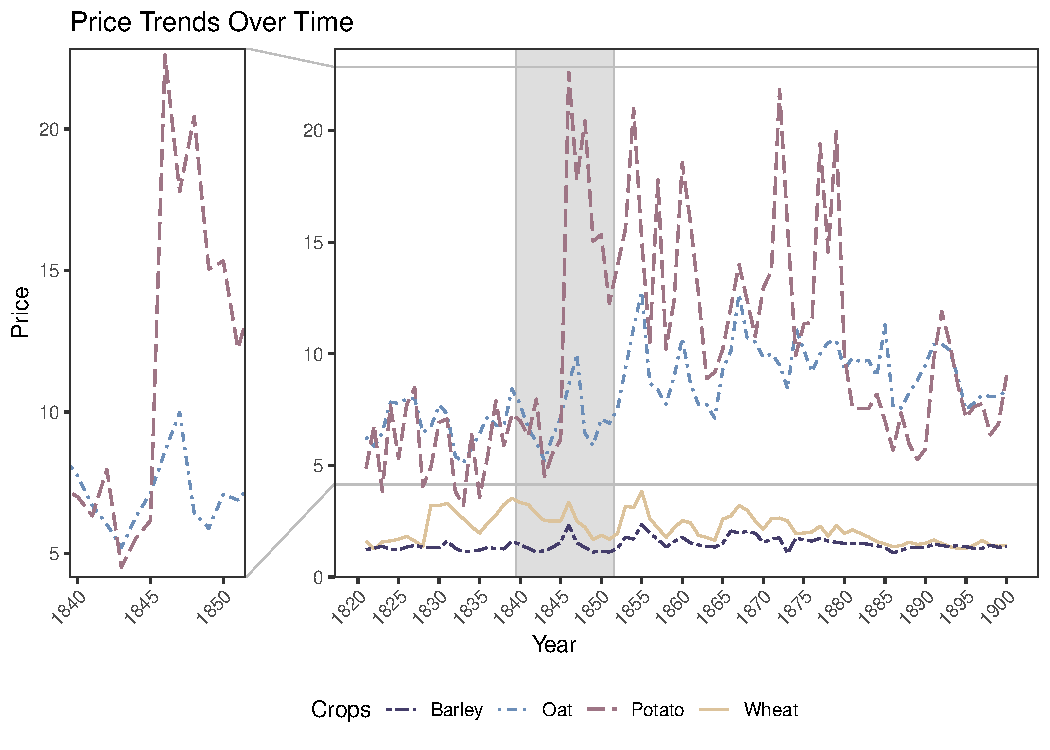
\includegraphics[width=.95\textwidth]{../03_outputs/grain_price.pdf}
\end{figure}

